
\documentclass[tikz,border=1pt]{standalone}

\usepackage{amsmath}
\usepackage{xcolor}
\usepackage{tikz}
\usetikzlibrary{calc, fit, matrix, positioning}

\tikzstyle{circ}=[circle, draw, minimum size=1.2cm]
\tikzstyle{square}=[rectangle, draw, minimum size=1cm]

\begin{document}

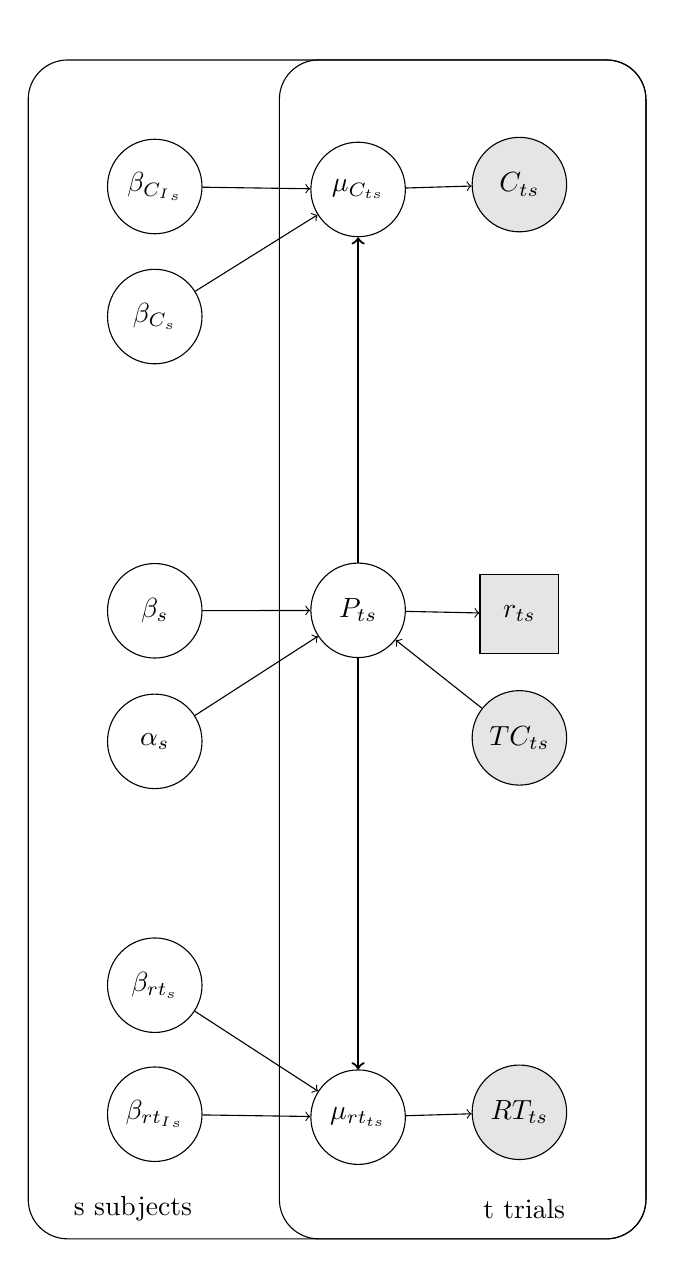
\begin{tikzpicture}
% Matrix m0
\matrix (m0) [
    ampersand replacement=\&,
    matrix of math nodes,
    nodes in empty cells,
    column sep=.3cm,
    row sep=0.4cm,
]
{
    \&  \& \& \&  \&\\
    \&  \& \& \&  \&  \&  \& \\
     |[circ]| \beta_{{C_I}_{s}}\&  \&  \& |[circ]| \mu_{{C}_{ts}} \& \&  |[circ, fill=gray!20]| C_{ts}  \\
    |[circ]| \beta_{{C}_{s}} \& \& \&   \&  \& \\
};

\draw[->] (m0-3-1) -- (m0-3-4);
\draw[->] (m0-4-1) -- (m0-3-4);
\draw[->] (m0-3-4) -- (m0-3-6);

% Matrix m1 (below m0)
\matrix (m1) [
    ampersand replacement=\&,
    matrix of math nodes,
    nodes in empty cells,
    column sep=.3cm,
    row sep=0.4cm,
    below=of m0
]
{
    \&  \& \& \& \&  \&  \& \\
    \&  \& \& \& \&  \&\\
    |[circ]| \beta_{s}\&  \&  \& |[circ]| P_{ts} \& \&  |[square, fill=gray!20]| r_{ts}  \\
    |[circ]| \alpha_{s} \& \& \&   \&  \& |[circ, fill=gray!20]| TC_{ts}\\
};

\draw[->] (m1-3-1) -- (m1-3-4);
\draw[->] (m1-4-1) -- (m1-3-4);
\draw[->] (m1-3-4) -- (m1-3-6);
\draw[->] (m1-4-6) -- (m1-3-4);
\draw[->, thick] (m1-3-4) -- (m0-3-4);

% Matrix m2 (below m1)
\matrix (m2) [
    ampersand replacement=\&,
    matrix of math nodes,
    nodes in empty cells,
    column sep=.3cm,
    row sep=0.4cm,
    below=of m1
]
{
    \&  \& \& \& \&  \&  \& \\
     |[circ]| \beta_{{rt}_{s}}\&  \&  \& \& \&   \\
    |[circ]| \beta_{{rt_I}_{s}}\& \& \& |[circ]| \mu_{{rt}_{ts}}\&  \& |[circ, fill=gray!20]| RT_{ts}\\
    \&  \& \& \& \&  \&\\
};

\draw[->] (m2-2-1) -- (m2-3-4);
\draw[->] (m2-3-1) -- (m2-3-4);
\draw[->] (m2-3-4) -- (m2-3-6);
\draw[->, thick] (m1-3-4) -- (m2-3-4);

% Plates
\pgfsetcornersarced{\pgfpoint{5mm}{5mm}}
\node[draw=black, fit=(m0-3-1) (m2-3-6), inner sep=10mm] {};
\pgfsetcornersarced{\pgfpoint{5mm}{5mm}}
% \node[draw=black, fit=(m0-3-4) (m2-3-6), inner sep=10mm] {};
\coordinate (adjusted_top) at ($(m0-3-4)+(0,6.45mm)$);
\node[draw=black, fit=(adjusted_top) (m2-3-6), inner sep=10mm] {};

\node[rotate=0, anchor=west] at (-4.0,-12.8) {s subjects};
\node[rotate=0, anchor=west] at (1.2,-12.8) {t trials};

\end{tikzpicture}

\end{document}
